\date{}
\title{}
\date{}
\begin{document}
\begin{frame}
    \titlepage
\end{frame}

\begin{frame}{last time}
    \begin{itemize}
    \item port numbers
    \item socket API
        \begin{itemize}
        \item socket address families, stream/datagram
        \item sendto/send, recvfrom/recv
        \item setsockopt
        \end{itemize}
    \item server socket concept
        \begin{itemize}
        \item bind() + listen() --- server socket
        \item accept(server socket) --- connection socket
        \end{itemize}
    \item TCP state machine
        \begin{itemize}
        \item three-way handshake (1 RTT before data)
        \item keeping sockets around in case of retransmission of connection-close ACKs
        \end{itemize}
    \item SO\_REUSEADDR
    \end{itemize}
\end{frame}

\section{broadcast}
\begin{frame}{broadcast/multicast}
\begin{itemize}
\item IPv4: can broadcast to every machine on local network
    \begin{itemize}
    \item set the SO\_BROADCAST socket option to 1
    \item send to special address 255.255.255.255 
    \item received at that port number on all machines
    \end{itemize}
\item multicast (send-to-many) groups
    \begin{itemize}
    \item request to receive: IP\_ADD\_MEMBERSHIP (v4), IPV6\_ADD\_MEMBERSHIP (v6)
    \item each `multicast group' has IP address
    \item 224.0.0.0/24 and ff02::/16 = local network only
    \item local network version usually implemented by broadcasting + filtering by IP
    \item (non-local-network multicast is more complex\ldots)
    \end{itemize}
\end{itemize}
\end{frame}

\begin{frame}{service discovery}
\begin{itemize}
\item example: find printers on local network automatically
\vspace{.5cm}
\item typical protocol mDNS (`multicast DNS')
\item uses IP addressses 224.0.0.251 / ff02::fb + port 5353
\item all machines on local network receive from all other machines on local network
\end{itemize}
\end{frame}


\section{aside: other address families}
\begin{frame}{other address families}
    \begin{itemize}
    \item AF\_UNIX {\small (= AF\_LOCAL in C, but not Python)}
        \begin{itemize}
        \item sockets can be represented in files on disk
        \item support sending file descriptors usually
        \end{itemize}
    \item (not sure how portable?) AF\_RAW
        \begin{itemize}
        \item usually how wireshark captures packets on Linux
        \item also supports writing packets
        \end{itemize}
    \item (Linux only) AF\_NETLINK 
        \begin{itemize}
        \item communicate with kernel networking code
        \end{itemize}
    \item AF\_AX25, AF\_APPLETALK, AF\_DECNET, \ldots
        \begin{itemize}
        \item other interesting protocols
        \end{itemize}
    \end{itemize}
\end{frame}


\section{URIs and URLs}
\begin{frame}{URL / URIs}
\begin{itemize}
\item Uniform Resource Locators (URL)
    \begin{itemize}
    \item tells how to find ``resource'' on network
    \item uniform --- one syntax for multiple protocols (types of servers, etc.)
    \end{itemize}
\item Unifrom Resources Identifiers
    \begin{itemize}
    \item superset of URLs
    \end{itemize}
\end{itemize}
\end{frame}

\begin{frame}[fragile]{URI examples}
\begin{Verbatim}[fontsize=\small,commandchars=X()]
https://kytos02.cs.virginia.edu:443/cs3130-spring2023/
                quizzes/quiz.php?qid=02#q2

https://kytos02.cs.virginia.edu/cs3130-spring2023/
                quizzes/quiz.php?qid=02

https://www.cs.virginia.edu/

sftp://cr4bd@portal.cs.virginia.edu/u/cr4bd/file.txt

tel:+1-434-982-2200

//www.cs.virginia.edu/~cr4bd/3130/S2023/
/~cr4bd/3130/S2023
    Xfbox(Xnormalfont scheme and/or host implied from context)
\end{Verbatim}
\end{frame}


\begin{frame}[fragile]{URI generally}
\begin{Verbatim}
scheme://authority/path?query#fragment
\end{Verbatim}
\begin{itemize}
\item scheme: --- what protocol
\item //authority/
    \begin{itemize}
    \item authoirty = user@host:port OR host:port OR user@host OR host
    \end{itemize}
\item path
    \begin{itemize}
    \item which resource
    \end{itemize}
\item ?query --- usually key/value pairs 
\item \#fragment --- place in resource
\vspace{.5cm}
\item most components (sometimes) optional
\end{itemize}
\end{frame}


\section{HTTP messages}
\usetikzlibrary{arrows.meta}
\begin{frame}{HTTP typical flow}
\begin{tikzpicture}
\tikzset{
    nodeline/.style={draw,ultra thick},
    msgline/.style={draw,very thick,-Latex},
    msgbox/.style={draw,fill=white,font=\small\tt,align=left},
}
\draw[nodeline] (0, -.5) -- ++(0, -7) node[pos=0,above] {client};
\draw[nodeline] (12, -.5) -- ++(0, -7) node[pos=0,above] {server};
\draw[msgline] (0, -1) -- (12, -2) node[midway,msgbox] {
    GET /~cr4bd/4457/F2024/ HTTP/1.1 \\
    Host: www.cs.virginia.edu \\
    \ldots
};
\draw[msgline] (12, -4) -- (0, -5) node[midway,above=-1cm,msgbox] {
    HTTP/1.1 200 OK \\
    Content-Type: text/html \\
    Content-Length: 5432 \\
    \ldots \\
    ~ \\
    <!DOCTYPE html\ldots
};
\draw[msgline] (0, -6) -- (12, -7) node[midway,msgbox] {
    GET /~cr4bd/4457/F2024/main.css HTTP/1.1 \\
    Host: www.cs.virginia.edu \\
    \ldots
};
\end{tikzpicture}
\end{frame}

\begin{frame}{HTTP message fields}
\begin{itemize}
\item requests:
    \begin{itemize}
    \item method (GET, HEAD, POST, \ldots) --- what to do
    \item URI (`path' and `query' part of URL, usually)
    \end{itemize}
\item responses:
    \begin{itemize}
    \item status code and message (200 OK, 404 Not Found, etc.)
    \end{itemize}
\item both:
    \begin{itemize}
    \item headers (key-value pairs)
    \item (sometimes) message body (arbitrary data)
    \end{itemize}
\end{itemize}
\end{frame}

\begin{frame}{HTTP/1.1 message format (RFC 2616)}
\begin{itemize}
\item ASCII text over TCP or TLS 
\item all newlines use `CRLF' (\textbackslash x0d\textbackslash x0a = \textbackslash r\textbackslash n)
\end{itemize}
\providecommand{\crlf}{\textit{\color{black!50}CRLF}}
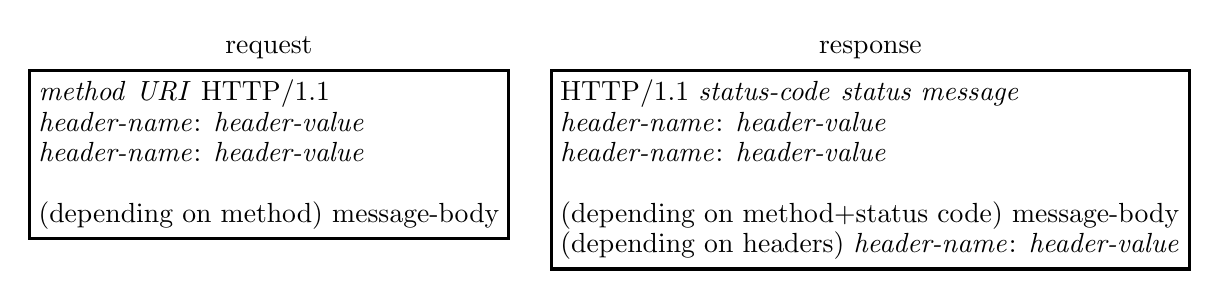
\begin{tikzpicture}
\node[draw,align=left,very thick,font=\fontsize{10}{11}\selectfont,label={north:request}] (request) {
\textit{method} \textit{URI} HTTP/1.1\\
\textit{header-name}: \textit{header-value} \\
\textit{header-name}: \textit{header-value} \\
~ \\
(depending on method) message-body
};
\node[anchor=north west,draw,align=left,font=\fontsize{10}{11}\selectfont,very thick,label={north:response}] 
at ([xshift=.5cm]request.north east){
HTTP/1.1 \textit{status-code} \textit{status message} \\
\textit{header-name}: \textit{header-value} \\
\textit{header-name}: \textit{header-value} \\
~ \\
(depending on method+status code) message-body \\
(depending on headers) \textit{header-name}: \textit{header-value}
};
\end{tikzpicture}
\end{frame}

\begin{frame}{HTTP/2, HTTP/3}
    \begin{itemize}
    \item `new' versions, not ubiquitously deployed
        \begin{itemize}
        \item HTTP/2: over TCP \textit{or} over TLS over TCP
        \item HTTP/3: over QUIC over UDP
        \end{itemize}
    \vspace{.5cm}
    \item multiple `streams' within one connection 
    \item send series of `frames' with stream ID + type + data
    \item frame types include:
        \begin{itemize}
        \item HEADERS --- encode message headers (key/value pairs)
        \item DATA --- include message bodies
        \end{itemize}
    \item method, status-code, URI encoded as special headers
    \end{itemize}
\end{frame}

\begin{frame}{HTTP/1.1 example (GET)}
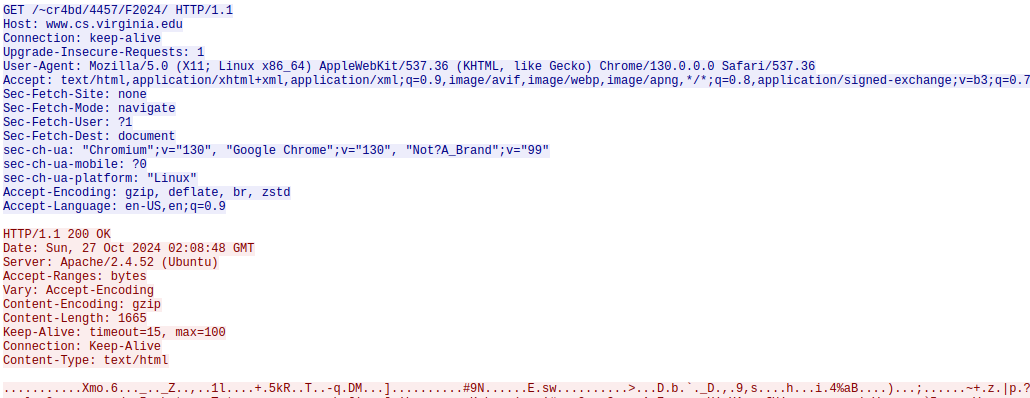
\includegraphics[width=\textwidth]{../http/http-wireshark-simple}
\end{frame}

\begin{frame}{HTTP/2.0 example (GET request)}
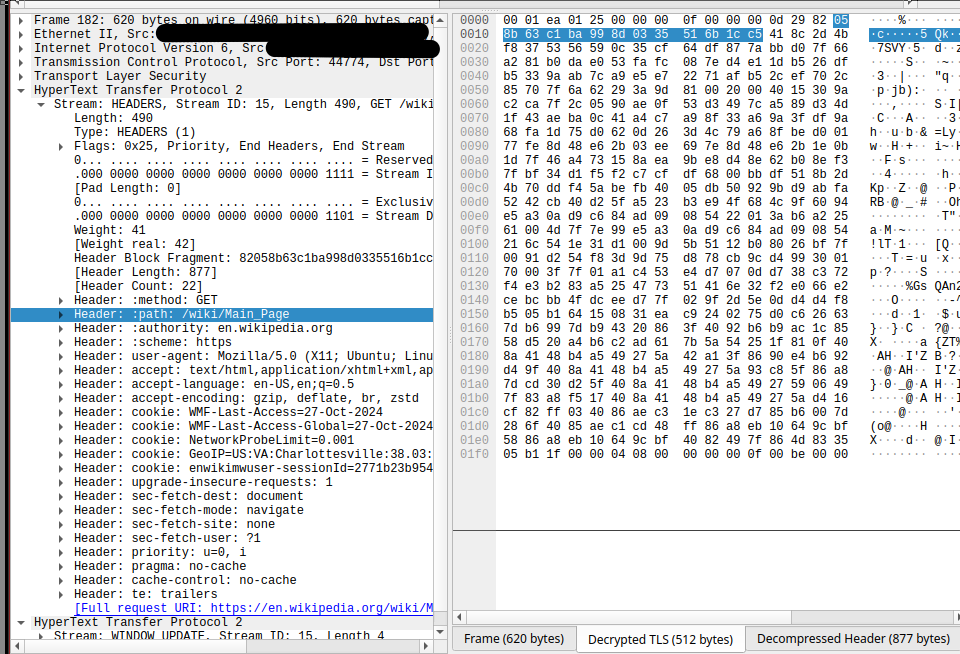
\includegraphics[width=\textwidth]{../http/http2-get-ex}
\end{frame}

% FIXME: HTTP/2.0 response

\begin{frame}{HTTP/1.1 example (POST)}
% FIXME
\end{frame}


\section{HTTP methods, briefly}
\begin{frame}{selected HTTP methods}
\small
\begin{tabular}{lllll}
method & purpose & request body? & respones body? & `safe' \\
GET & retrieve resource & never & usually & yes \\
HEAD & retrieve resource headers& never & never & yes \\
POST & provide data & always & usually & no \\
PUT & set contents of resource & always & maybe & no \\
DELETE & delete resource & never & maybe & no \\
OPTIONS & get info about server & maybe & maybe & no \\
\end{tabular}
\end{frame}

\begin{frame}{safety}
    \begin{itemize}
    \item GET, HEAD = `safe' methods
    \item okay for clients to repeat, send unprompted
        \begin{itemize}
        \item `prefetch' resources
        \item redo when user presses back button unprompted
        \end{itemize}
    \item other methods: that's not okay!
    \end{itemize}
\begin{center}
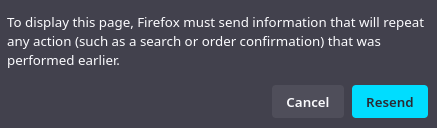
\includegraphics[width=0.7\textwidth]{../http/ff-resend-warning}
\end{center}
\end{frame}



\section{HTTP POST}
\begin{frame}[fragile]{HTTP POST}
\begin{Verbatim}[fontsize=\small]
POST /cs4457-fall2024-quiz-listener.php HTTP/1.1
Host: kytos02-noauth.cs.virginia.edu
Content-Type: application/json
Content-Length: 184
...

{"user":"cr4bd","realuser":"cr4bd","session_id":"abcdefabcdef0123456789aaaaaaaaaaaaaaaaaaaaaaaaaaaaaaaaaaaaaaaaaa","quiz":"week09","slug":"71d45222","answer":["d2f4e81b"],"sequence":0}
\end{Verbatim}
\end{frame}

\begin{frame}[fragile]{HTML forms (GET)}
\begin{tikzpicture}
\node[align=left,font=\fontsize{8}{9}\selectfont] (html) {
\begin{minipage}{0.6\textwidth}
\begin{Verbatim}
<form action="https://example.com/foo" method="get">
Name: <input type="text" name="name"><br>
Query: <input type="text" name="query"><br>
<input type="submit" value="Submit">
</form>
\end{Verbatim}
\end{minipage}
};
\node[anchor=north east] (pic) at (html.north west) {
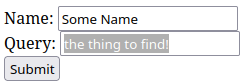
\includegraphics[width=0.3\textwidth]{../http/html-form-get.png}
};
\end{tikzpicture}
\begin{Verbatim}[fontsize=\small]
GET /foo?name=Some+Name&query=the+thing+to+find%21 HTTP/1.1
Host: example.com
...
\end{Verbatim}
\end{frame}

\begin{frame}[fragile]{HTML forms (POST)}
\begin{tikzpicture}
\node[align=left,font=\fontsize{8}{9}\selectfont] (html) {
\begin{minipage}{0.6\textwidth}
\begin{Verbatim}
<form action="https://example.com/foo" method="post">
Name: <input type="text" name="name"><br>
Comment:
<textarea name="comment">
</textarea>
<br>
<input type="submit" value="Submit">
</form>
\end{Verbatim}
\end{minipage}
};
\node[anchor=north east] (pic) at (html.north west) {
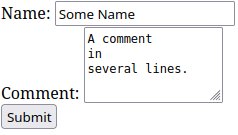
\includegraphics[width=0.3\textwidth]{../http/html-form-post.png}
};
\end{tikzpicture}
\begin{Verbatim}[fontsize=\small]
POST /foo HTTP/1.1
Host: example.com
Content-Type: application/x-www-form-urlencoded
Content-Length: 60
...

name=Some+Name&comment=A+comment%0D%0Ain%0D%0Aseveral+lines.
\end{Verbatim}
\end{frame}

\begin{frame}[fragile]{HTML forms (multipart/form-data)}
\begin{Verbatim}[fontsize=\fontsize{9}{10}]
<form action="https://example.com/foo" method="post"
    enctype="multipart/form-data">
    ...
\end{Verbatim}
\rule{0.9\textwidth}{1mm}
\begin{Verbatim}[fontsize=\fontsize{9}{10}]
POST /foo HTTP/1.1
Host: example.com
Content-Type: multipart/form-data; boundary=---------------------------81545828010202052201987031310
Content-Length: 321
...

-----------------------------30871118663472832060210928793
Content-Disposition: form-data; name="name"

Some Name
-----------------------------30871118663472832060210928793
Content-Disposition: form-data; name="comment"

A comment
in
several lines.
-----------------------------30871118663472832060210928793--
\end{Verbatim}
\end{frame}

\begin{frame}{GET v POST}
\begin{tabular}{p{7cm}|p{7cm}}
GET & POST \\ \hline
works with back button, caches & not resent automatically \\
limited by URL size & huge possible size \\
saving URL accesses page again & form info never `leaked' in browser history, referer, etc.\\
only simple text fields & supports file uploads (via multipart/form-data) \\
\end{tabular}
\end{frame}



\section{exercise: HTTP which}
\begin{frame}{exercise: which method}
    \begin{itemize}
    \item GET or POST or something else for
    \vspace{.5cm}
    \item image that shows a clock with current time
    \item rating a product and displaying the resulting summary of all ratings
    \item search query for a Twitter-like website
    \item getting the 2nd page of search results
    \end{itemize}
\end{frame}


\section{virtual hosting, Host header}
\begin{frame}[fragile]{multiple names, one IP}
\begin{Verbatim}
$ dig +short es.wikipedia.org aaaa
dyna.wikimedia.org.
2620:0:860:ed1a::1
$ dig +short en.wikipedia.org aaaa
dyna.wikimedia.org.
2620:0:860:ed1a::1
\end{Verbatim}
\begin{itemize}
\item how does this work?
\end{itemize}
\end{frame}

\begin{frame}{Host/:authority header}
\begin{itemize}
\item when getting http://somehostname/path, send header
\item \texttt{Host: somehostname} (HTTP/1.1)
\item \texttt{:authority: somehostname} (HTTP/2, HTTP/3)
\vspace{.5cm}
\item allows for `virtual hosts'
\end{itemize}
\end{frame}


\section{error codes}
\begin{frame}{selected HTTP status codes}
\begin{itemize}
\item 1xx --- informational
\item 2xx --- successful
    \begin{itemize}
    \item 200 OK, 204 No Content
    \end{itemize}
\item 3xx --- redirection
    \begin{itemize}
    \item 301 Moved Permanently, 302 Found, 303 See Other
    \item `Location' header gives next URL to use
    \item 304 Not Modified (conditional GET --- later)
    \end{itemize}
\item 4xx --- client error
    \begin{itemize}
    \item 403 Forbidden, 404 Not Found
    \end{itemize}
\item 5xx --- server error
\end{itemize}
\end{frame}

% FIXME

\section{persistent, pipelining}
% FIXME: pipelining screenshot
\begin{frame}{one connection, multiple requests}
    \begin{itemize}
    \item HTTP/0.9, HTTP/1.0 --- one request+response per connection
        \begin{itemize}
        \item big efficiency problem
        \end{itemize}
    \item solution 1: persistent connections
    \item solution 2: pipelining
    \item solution 3 (HTTP/2+): multiple `streams' in one connection
    \end{itemize}
\end{frame}

\begin{frame}{end-of-request/response}
    \begin{itemize}
    \item body of request/response can be variable length
    \vspace{.5cm}
    \item so when does request/response end if it has a body?
    \item HTTP/1.0 original solution (RFC 1945)
        \begin{itemize}
        \item ``the length of that body may be determined in two ways. If a Content-Length field is present, the value in bytes represents the length of the Entity-Body. Otherwise, the body length is determined by the closing of the connection by the server.''
        \end{itemize}
    \item advantage of latter idea: don't need to generate whole document before sending headers
    \item disadvantage: no persistent connections!
    \end{itemize}
\end{frame}


\providecommand{\chunksize}[1]{\textbf{\color{violet!80}#1}}
\begin{frame}[fragile,label=chunked]{chunked transfer coding}
\begin{Verbatim}[commandchars=\\\{\}]
HTTP/1.1 200 OK
Content-Type: text/plain
\textbf{Transfer-Coding: chunked}
...

\chunksize{1B}
\textbf{This is 0x1B bytes of text.}
\chunksize{21}
\textbf{And 0x21 bytes}
\textbf{with more lines.}
\chunksize{0}
\end{Verbatim}
\end{frame}

\begin{frame}{pipelining}
\begin{tikzpicture}
\tikzset{
    nodeline/.style={draw,ultra thick},
    msgline/.style={draw,very thick,-Latex},
    msgbox/.style={draw,fill=white,font=\small\tt,align=left},
}
\draw[nodeline] (0, -.5) -- ++(0, -7) node[pos=0,above] {client};
\draw[nodeline] (12, -.5) -- ++(0, -7) node[pos=0,above] {server};
\draw[msgline] (0, -1) -- (12, -2) node[midway,msgbox] {
    GET /image1.png HTTP/1.1
    \ldots
};
\draw[msgline] (0, -1.5) -- (12, -2.5) node[midway,msgbox] {
    GET /image2.png HTTP/1.1
    \ldots
};
\draw[msgline] (0, -2) -- (12, -3) node[midway,msgbox] {
    GET /script.js HTTP/1.1
    \ldots
};
\draw[msgline] (12, -2.5) -- (0, -3) node[midway,below,msgbox] {
    HTTP/1.1 200 OK
    \ldots
};
\draw[msgline] (12, -4) -- (0, -5) node[midway,msgbox] {
    HTTP/1.1 200 OK
    \ldots
};
\draw[msgline] (12, -5) -- (0, -6) node[midway,msgbox] {
    HTTP/1.1 200 OK
    \ldots
};
\end{tikzpicture}
\end{frame}

\begin{frame}{HTTP/1.1 `pipelining'}
    \begin{itemize}
    \item send series of requests before receiving any response
    \item potentailly server can potentially process requests in parallel
    \vspace{.5cm}
    \item need to handle resending requests if connection dropped early
    \end{itemize}
\end{frame}

\begin{frame}{HTTP/2.0 multiple streams}
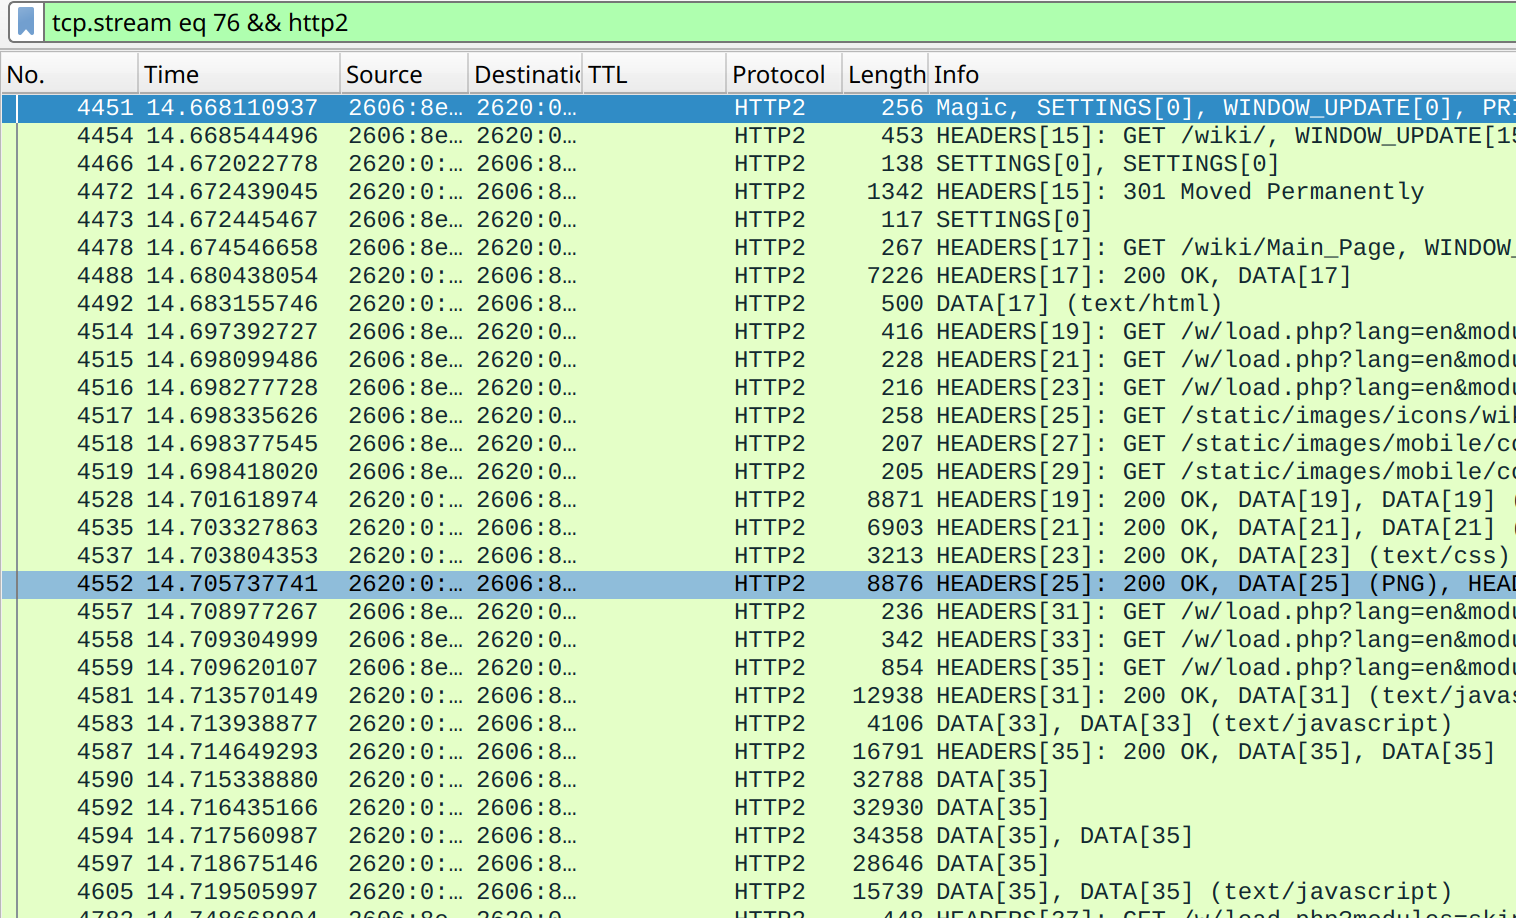
\includegraphics[width=\textwidth]{../http/http2-multi-reqres}
\end{frame}


\section{content negotiation}
\begin{frame}{content negotiation}
\begin{itemize}
\item Firefox on my desktop $\rightarrow$ wikipedia:
\item {\small\texttt{accept: text/html,application/xhtml+xml,application/xml;q=0.9,image/avif,image/webp,image/png,image/svg+xml,*/*;q=0.8}}
    \begin{itemize}
    \item list of formats and preference indicator for each (\texttt{q})
    \item described using ``media types'' (RFC 6838)
    \end{itemize}
\item {\small\texttt{accept-language: en-US,en;q=0.5}}
\item {\small\texttt{accept-encoding: gzip, deflate, br, zstd}}
    \begin{itemize}
    \item allowed compression formats
    \end{itemize}
\end{itemize}
\end{frame}

\begin{frame}{advice against content negotation}
\begin{itemize}
\item current HTTP standard (RFC 9110) says this approach ``has several disadvantages'':
    \begin{itemize}
    \item advises considering approaches where client chooses version
    \end{itemize}
\item `impossible for the server to accurately determine what might be ``best'' '
\item `having the [client] describe its capabilities in every request can be very inefficient \ldots and a potential risk to the user's privacy'
\item `complicates the implementation'
\item `limits \ldots shared caching'
\end{itemize}
\end{frame}


\section{cookies}
\begin{frame}{HTTP non-state}
    \begin{itemize}
    \item HTTP is a `stateless'
    \item each request stands on its own
        \begin{itemize}
        \item processed independently of all other requests
        \item even if multiple in a connection
        \end{itemize}
    \vspace{.5cm}
    \item this is disappointing for websites: \\
    supporting `login' functionality \\
    supporting user preferences
    \end{itemize}
\end{frame}

\begin{frame}[fragile]{HTTP cookies (RFC 6265)}
example.com $\rightarrow$ client
\begin{Verbatim}[fontsize=\small]
HTTP/1.1 200 OK
Set-Cookie: SessionID=31d4d96e407aad42; Path=/; Domain=example.com
\end{Verbatim}
client $\rightarrow$ example.com on later requests:
\begin{Verbatim}[fontsize=\small]
GET /some-path HTTP/1.1
Host: example.com
Cookie: SessionID=31d4d96e407aad42
\end{Verbatim}
\end{frame}


\begin{frame}{session ID concept}
    \begin{itemize}
    \item assign random ID number to each `session' if no cookie set
    \vspace{.5cm}
    \item in some database:
    \item if they add to shopping cart, associate ID number with shopping cart items
    \item if user logs in, associate ID number with user
    \item \ldots
    \end{itemize}
\end{frame}

\begin{frame}{selected cookie attributes}
\begin{itemize}
\item domain --- limit to subset of domains
    \begin{itemize}
    \item domain=example.com matches example.com, foo.example.com, but not other.com
    \end{itemize}
\item secure --- only send back on encrypted connections
\item httponly --- do not expose to in-webpage scripts
\item expires, max-age --- limit how long cookie kept around
    \begin{itemize}
    \item default = until browser closed
    \end{itemize}
\end{itemize}
\end{frame}

\begin{frame}{cookies and tracking}
    \begin{itemize}
    \item cookies often used for tracking users \textit{across websites}
    \item and not by setting cookies valid for tons of domains
    \vspace{.5cm}
    \item how: websites load data from other websites
        \begin{itemize}
        \item separate HTTP requests with separate cookies
        \end{itemize}
    \end{itemize}
\end{frame}

\begin{frame}{cookie tracking example}
\begin{itemize}
\item foo.com, bar.com, quux.com all include an image
    \begin{itemize}
    \item https://tracker.com/track-XXX.png where XXX is foo, bar or quux
    \end{itemize}
\item tracker.com can read cookie every time image is accessed
    \begin{itemize}
    \item and set a cookie to unique number if not set
    \end{itemize}
\item now tracker.com knows:
    \begin{itemize}
    \item when/if every visitor of foo.com visited bar.com and/or quux.com
    \end{itemize}
\end{itemize}
\end{frame}

\begin{frame}{more detailed tracking?}
    \begin{itemize}
    \item ``just'' learned about how many visitors visited combinations of websites
    \item with some cooperation can get more info:
        \begin{itemize}
        \item which subpages on those websites
        \item username or email entered into those websites
        \item \ldots
        \end{itemize}
    \item one way to pass info: add extra data to image filename
    \end{itemize}
\end{frame}

\begin{frame}{third party cookie rules}
    \begin{itemize}
    \item some browsers might restrict `third-party cookies'
        \begin{itemize}
        \item cookies sent to Y because of visit to X
        \end{itemize}
    \item various options, with variable deployment:
        \begin{itemize}
        \item only make third-party cookies work if marked SameSite=None
        \item separate cookie storage for each `root' website
        \item ignore cookies from unvisited sites
        \item disable only cookies that heuristically look like tracking
        \end{itemize}
    \end{itemize}
\end{frame}


\section{caching}
\begin{frame}{HTTP caching (RFC 9111)}
    \begin{itemize}
    \item making webpages fast --- let clients cache values for later
    \item some problems:
    \vspace{.5cm}
    \item how to tell if something's out of date
    \item how to tell if changes to cookies/accept-language/etc. change item
    \end{itemize}
\end{frame}

\begin{frame}<1>[label=oodOpt]{is it out of date? options}
    \begin{itemize}
    \item \myemph<2>{expire date; max-age in seconds}
    \item \myemph<3>{check with server if it has changed}
    \end{itemize}
\end{frame}

\againframe<2>{oodOpt}

\begin{frame}[fragile]{expires}
\begin{Verbatim}
HTTP/1.1 200 OK
Date: Mon, 28 Oct 2024 00:29:02 GMT
Expires: Mon, 28 Oct 2024 04:29:02 GMT
...
\end{Verbatim}
\rule{0.9\textwidth}{1mm}
\begin{Verbatim}
HTTP/1.1 200 OK
Cache-Control: max-age=14400
...
\end{Verbatim}
\end{frame}

\againframe<3>{oodOpt}

\begin{frame}[fragile]{conditional GETs}
\begin{Verbatim}[fontsize=\fontsize{12}{13}]
GET /3/library/struct.html HTTP/1.1
...

HTTP/1.1 200 OK
Date: Sun, 27 Oct 2024 20:01:15 GMT
Last-Modified: Sun, 27 Oct 2024 18:50:46 GMT
ETag: "671e8b86-13e32"
\end{Verbatim}
\rule{0.9\textwidth}{1mm}
\begin{Verbatim}[fontsize=\fontsize{12}{13}]
GET /3/library/struct.html HTTP/1.1
If-Modified-Since: Sun, 27 Oct 2024 18:50:46 GMT
If-None-Match: "671e8b86-13e32"
...
HTTP/1.1 304 Not Modified
...
\end{Verbatim}
\end{frame}

\begin{frame}[fragile]{variable responses}
\begin{Verbatim}
HTTP/1.1 200 OK
...
Vary: Accept, Accept-Lnaguage, Cookie
...
\end{Verbatim}
\begin{itemize}
\item page contents may vary even though URL doesn't change
\item Vary header says what things need to be the same
\item typically used to discard cached responses
\end{itemize}
\end{frame}

\begin{frame}[fragile]{other cache-control settings}
\begin{itemize}
\item seen max-age=X, also\ldots
\item no-store
    \begin{itemize}
    \item do not store a copy of this response
    \end{itemize}
\item no-cache
    \begin{itemize}
    \item do not use without checking for new version first (conditional GET or similar)
    \end{itemize}
\item private, public
    \begin{itemize}
    \item indicate if acceptable for cache shared between users
    \end{itemize}
\end{itemize}
\end{frame}


\section{proxies and reverse proxies}
\usetikzlibrary{arrows.meta}
\begin{frame}{HTTP proxies (1)}
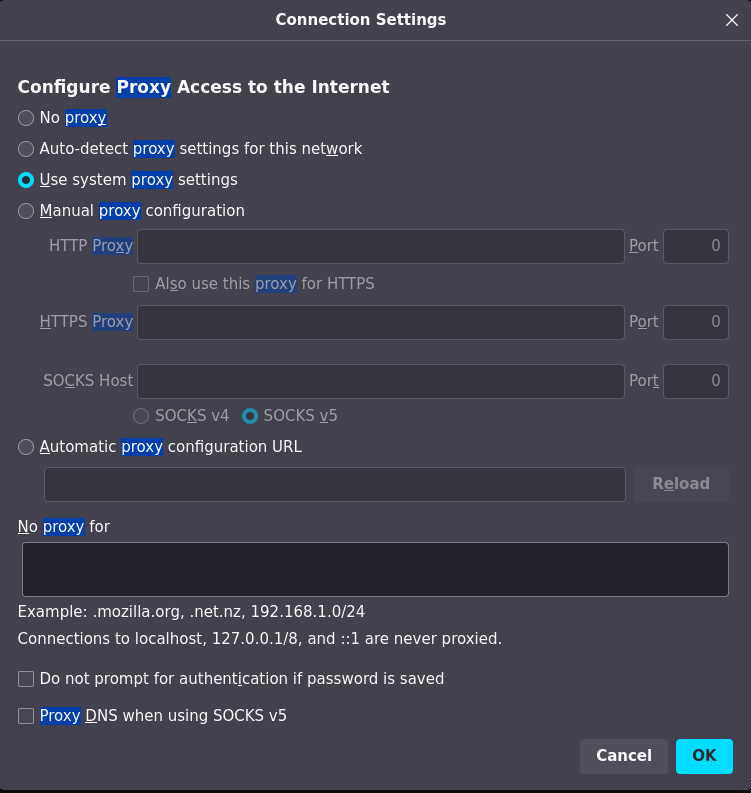
\includegraphics[height=0.9\textheight]{../http/moz-proxy-config}
\end{frame}

\begin{frame}
\begin{tikzpicture}
\node[draw, very thick,align=center] (user agent) at (0, 0) {
    user-agent \\ (example: \\ web browser)
};
\node[draw, very thick,align=center] (proxy) at (6, 0) {
    proxy \\server
};
\node[draw, very thick,align=center] (web server) at (12, 0) {
    web \\server
};
\draw[thick,Latex-Latex] (user agent) -- (proxy)
    node[pos=0,above right] {client}
    node[pos=1,above left] {server}
    coordinate[midway] (midpt cp);
\draw[thick,Latex-Latex] (proxy) -- (web server)
    node[pos=0,above right] {client}
    node[pos=1,above left] {server}
    coordinate[midway] (midpt ps);
\draw (midpt cp) -- ++(0cm, -1cm) node[below,align=center] {
    request specifies \\
    which web server \\
    to contact
};
\draw (midpt ps) -- ++(0cm, -1cm) node[below,align=center] {
    looks like normal \\
    user-agent request 
};
\end{tikzpicture}
\end{frame}

\begin{frame}[fragile]{HTTP proxies (2)}
browser$\rightarrow$HTTP(S) proxy sever: \\
\begin{Verbatim}
GET http://example.com/somesite HTTP/1.1
Host: example.com
...
\end{Verbatim}
\rule{.9\textwidth}{1mm}
\begin{itemize}
    \item instead of path, can put full URL
    \item doesn't have to be \texttt{http} URL
\end{itemize}
\end{frame}

\begin{frame}{proxy functionality}
    \begin{itemize}
    \item caching for multiple users
        \begin{itemize}
        \item reason for \texttt{Cache-Control: private}
        \end{itemize}
    \item filtering content
        \begin{itemize}
        \item antimalware, adblocking, etc.
        \end{itemize}
    \item logging content (example: debugging webapp)
    \item \ldots
    \end{itemize}
\end{frame}

\begin{frame}
\begin{tikzpicture}
\node[draw, very thick,align=center] (user agent) at (0, 0) {
    user-agent \\ (example: \\ web browser)
};
\node[draw, very thick,align=center] (proxy) at (6, 0) {
    forward proxy \\server
};
\node[draw, very thick,align=center] (web server) at (12, 0) {
    web \\server
};
\draw[thick,Latex-Latex] (user agent) -- (proxy)
    node[pos=0,above right] {client}
    node[pos=1,above left] {server}
    coordinate[midway] (midpt cp);
\draw[thick,Latex-Latex] (proxy) -- (web server)
    node[pos=0,above right] {client}
    node[pos=1,above left] {server}
    coordinate[midway] (midpt ps);
\draw (midpt cp) -- ++(0cm, -1cm) node[below,align=center] {
    request specifies \\
    which web server \\
    to contact
};
\draw (midpt ps) -- ++(0cm, -1cm) node[below,align=center] {
    looks like normal \\
    user-agent request 
};

\begin{scope}[yshift=-5cm,name prefix=rvs-]
\node[draw, very thick,align=center] (user agent) at (0, 0) {
    user-agent \\ (example: \\ web browser)
};
\node[draw, very thick,align=center] (proxy) at (6, 0) {
    reverse proxy \\server
};
\node[draw, very thick,align=center] (web server) at (12, 0) {
    backend\\server
};
\draw[thick,Latex-Latex] (user agent) -- (proxy)
    node[pos=0,above right] {client}
    node[pos=1,above left] {server}
    coordinate[midway] (midpt cp);
\draw[thick,Latex-Latex] (proxy) -- (web server)
    node[pos=0,above right] {client}
    node[pos=1,above left] {server}
    coordinate[midway] (midpt ps);
\draw (midpt cp) -- ++(0cm, -1cm) node[below,align=center] {
    looks like normal \\
    user-agent request
};
\draw (web server) -- ++(-1cm, -1cm) node[below,align=center] {
    selected from \\
    user-agent request path
};
\end{scope}
\end{tikzpicture}
\end{frame}

\begin{frame}{reverse proxy}
    \begin{itemize}
    \item why not just go directly to actual web server?
    \vspace{.5cm}
    \item make multiple web severs appear as one? example:
        \begin{itemize}
        \item https://example.com/foo/XXX goes to https://foo-backend.example.com/XXX
        \item https://example.com/bar/XXX goes to https://bar-backend.example.com/XXX
        \item https://example.com/ goes to https://frontpage.example.com/
        \end{itemize}
    \item do caching, filtering, or similar on behalf of webservers
    \item split requests between multiple identical servers for performance
    \end{itemize}
\end{frame}


\subsection{aside: wikimedia architecture}
\begin{frame}{Wikimedia architecture}
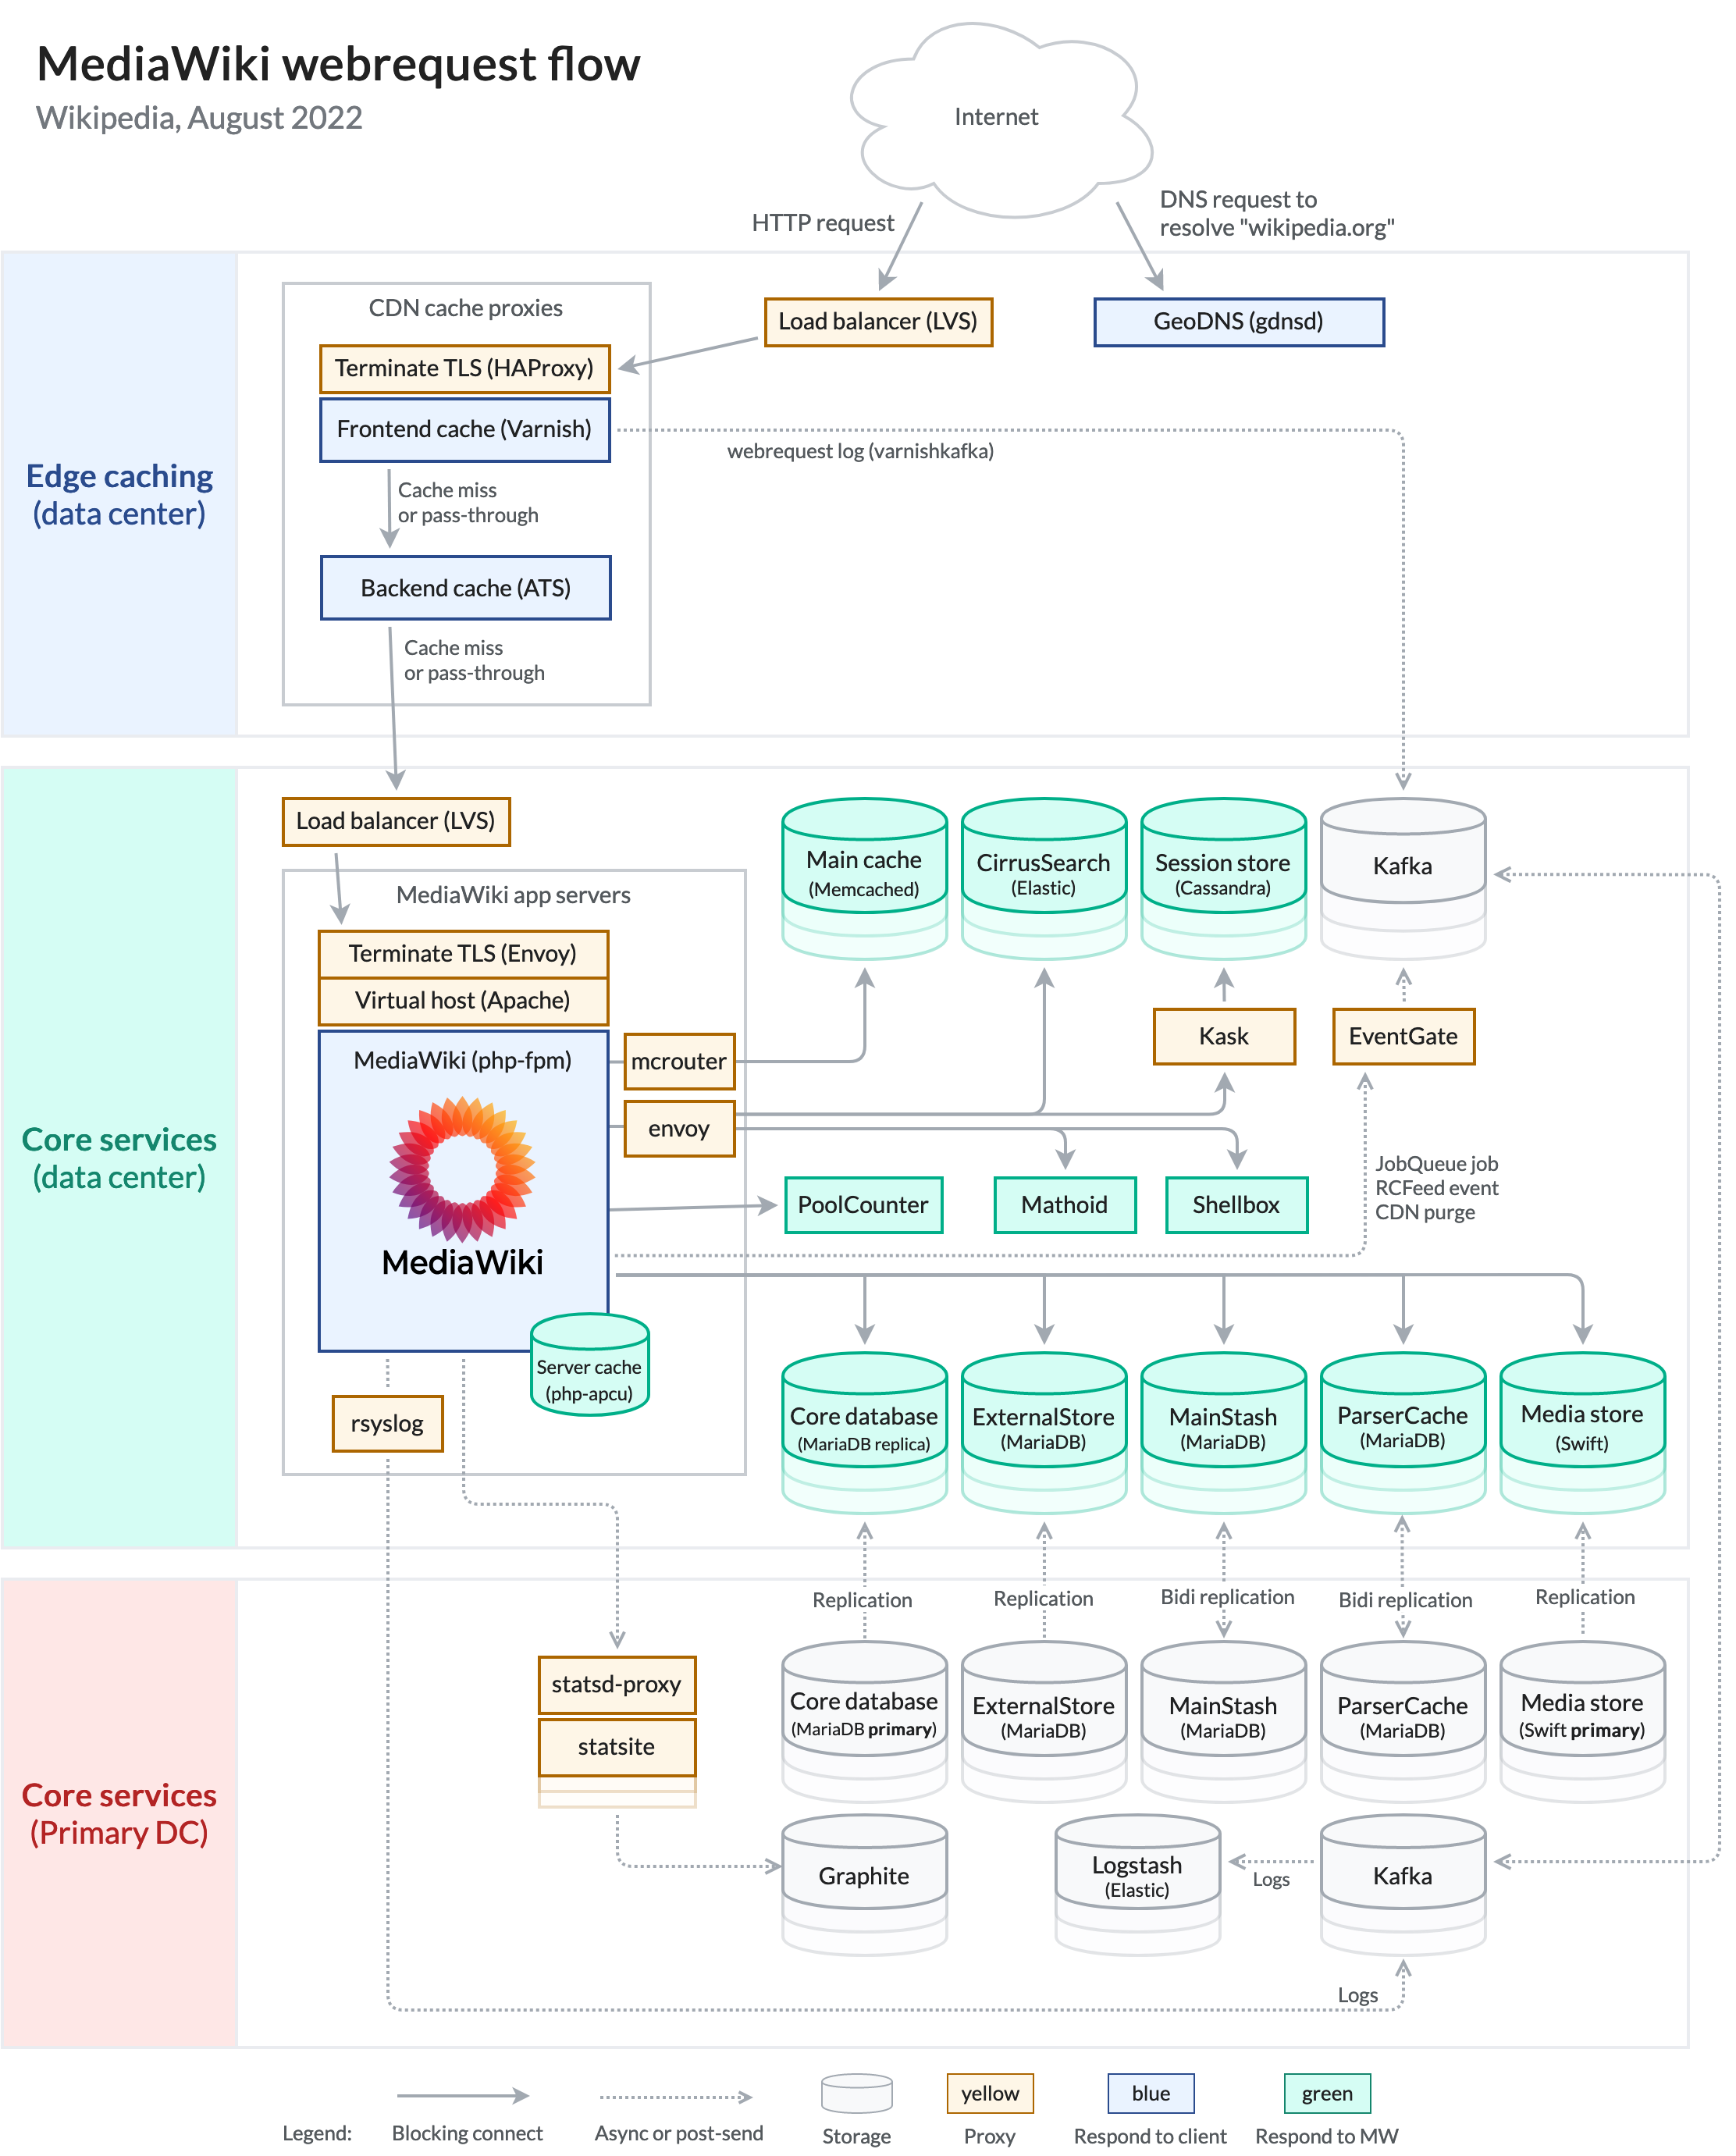
\includegraphics[height=0.85\textheight]{../http/Wikipedia_webrequest_2022.png}
\end{frame}


\section{REST}
\begin{frame}{REST}
    \begin{itemize}
    \item REpresentational State Transfer
    \item idea for application interface on top of HTTP
    \vspace{.5cm}
    \item entities in system represented with URLs
    \item GET requests to get state of that entity
    \item PUT and/or POST requests to update entity state
    \item DELETE requests to remove entity
    \end{itemize}
\end{frame}

\begin{frame}[fragile]{example: Canvas API for announcements (1)}
client $\rightarrow$ canvas HTTP server:
\begin{Verbatim}[fontsize=\fontsize{9}{10}\selectfont]
GET /api/v1/courses/123456/discussion_topics?only_announcements=true
Authorization: Bearer [secret code]
\end{Verbatim}
\rule{0.9\textwidth}{1mm}
\begin{Verbatim}[fontsize=\fontsize{9}{10}\selectfont]
HTTP/1.1 200 OK
...

[{
    "id":1,
    "title":"Welcome to the Course!",
    "message":"...",
    ...
},
{
    "id":2,
    ...
\end{Verbatim}
\end{frame}

\begin{frame}[fragile]{example: Canvas API for announcements (2)}
client $\rightarrow$ canvas HTTP server:
\begin{Verbatim}[fontsize=\fontsize{9}{10}\selectfont]
POST /api/v1/courses/123456/discussion_topics
Authorization: Bearer [secret code]
Content-Type: application/json
...

{
    "is_announcement":true,
    "title":"Class Cancelled",
    "message":"....."
}
\end{Verbatim}
\rule{0.9\textwidth}{1mm}
\begin{Verbatim}[fontsize=\fontsize{9}{10}\selectfont]
HTTP/1.1 200 OK
...

{
    "id": 41,
    "title":"Class Cancelled",
    ....
}
\end{Verbatim}
\end{frame}

\begin{frame}[fragile]{example: Canvas API for announcements (3)}
client $\rightarrow$ canvas HTTP server:
\begin{Verbatim}[fontsize=\fontsize{9}{10}\selectfont]
PUT /api/v1/courses/123456/discussion_topics/41
Authorization: Bearer [secret code]
Content-Type: application/json
...

{
    "is_announcement":true,
    "title":"Class Cancelled [updated!]",
    "message":"UPDATE: prevoiusly,.."
    ...
}
\end{Verbatim}
\rule{0.9\textwidth}{1mm}
\begin{Verbatim}[fontsize=\fontsize{9}{10}\selectfont]
HTTP/1.1 200 OK
...

{
    "id": 41,
    "title":"Class Cancelled [updated!]",
    ....
}
\end{Verbatim}
\end{frame}



% FIXME: SOAP? HLS?


\section{backup slides}
\begin{frame}{backup slides}
\end{frame}

\section{cache poisoning}
% spoofing protections
    % port numbers, IDs, capitalization, TCP

\usetikzlibrary{arrows.meta,calc,fit,matrix,shapes,shapes.misc}
\providecommand{\computer}{%
    
\includegraphics[width=1cm]{../common/Noun_project_216.pdf}
}
\providecommand{\computerAlt}{%
    
\includegraphics[width=1cm]{../common/Noun_project_alt_cpu.pdf}
}
\providecommand{\switch}{%
    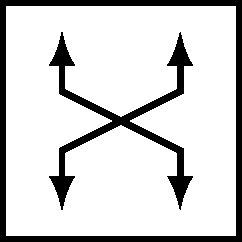
\includegraphics[width=0.9cm]{../common/fig-switch.pdf}
}
\providecommand{\router}{%
    
\includegraphics[width=0.9cm]{../common/fig-router.pdf}
}


\begin{frame}{DNS cache poisoning}
\begin{tikzpicture}
\tikzset{
    computer/.style={inner sep=0mm,outer sep=0mm,execute at begin node={\computer}},
    computer alt/.style={inner sep=0mm,outer sep=0mm,execute at begin node={\computerAlt}},
    connect/.style={draw,very thick,Latex-Latex},
    connect big/.style={draw,ultra thick,Latex-Latex},
    network/.style={cloud,draw,aspect=2},
    marked/.style={draw,line width=1mm,blue,dotted},
    marked pack/.style={draw,solid,line width=0.8mm,draw=blue,fill=white,align=left,
        font=\small},
    marked alt/.style={draw,line width=1mm,violet,dotted},
    marked pack alt/.style={draw,solid,line width=0.8mm,draw=violet,fill=white,align=left,
        font=\small},
};

\node[computer] (attacker) at (0, 2) {};
\node[computer] (attacker2) at (0, -4) {};
\node[font=\huge] at (attacker) {\emoji{smiling-face-with-horns}};
\node[font=\huge] at (attacker2) {\emoji{smiling-face-with-horns}};
\node[computer] (victim) at (0, -2) {};
\node[network] (net) at (3.5, 0) {~~};
\node[network] (net2) at (5, -4) {~~};
\node[computer,label={south:dns.isp.com}] (resolver) at (7, 2) {};
\node[computer,label={south:ns.foo.com}] (authority) at (10, -4) {};
%
\draw[connect] (attacker) -- (net);
\draw[connect] (victim) -- (net);
\draw[connect] (net) -- (net2);
\draw[connect] (net) -- (resolver);
\draw[connect] (net2) -- (authority);
\draw[connect] (net2) -- (attacker2);
%
\begin{visibleenv}<2>
\draw[marked,-Latex] (attacker) -- ([yshift=.1cm]net.center) 
    node[pos=0.25,above right,marked pack] {
        \emoji{smiling-face-with-horns} user $\rightarrow$ dns.isp.com: \\
        foo.com IN A ?
    } -- (resolver.west);
\end{visibleenv}
\begin{visibleenv}<3>
\draw[marked,-Latex] (resolver.south) -- ([yshift=-.1cm]net.center) 
    node[pos=0.25,above right,marked pack] {
        dns.isp.com $\rightarrow$ ns.foo.com: \\
        foo.com IN A ?
    } -- (net2.center) -- (authority);
\end{visibleenv}
\begin{visibleenv}<3>
\draw[marked,-Latex] (attacker2) -- (net2.center)
    node[pos=0.25,marked pack,above right] {
        ns.foo.com $\rightarrow$ dns.isp.com: \\
        foo.com 9999999 IN A (attcker's IP) 
    }
    -- ([yshift=-.2cm]net.center) -- ([yshift=-.2cm]resolver.west);
\node[anchor=north west,draw=red,ultra thick,align=left,font=\small] at ([xshift=2cm]resolver.north east) {
    attacker's `spoofed' response \\
    causes dns.isp.com to record \\
    wrong IP
};
\end{visibleenv}
\begin{visibleenv}<4>
\draw[marked,-Latex] (victim) -- (net) node[pos=0.25,above right,marked pack] {
       innocent user $\rightarrow$ dns.isp.com: \\
       foo.com IN A ?
}
    -- (resolver.west);

\draw[marked,-Latex] (resolver.south) -- (net) node[pos=0.25,above right,marked pack] {
       dns.isp.com $\rightarrow$  dns.isp.com: \\
       foo.com 9999944 IN A (attacker's IP)
    }
    -- (victim);
\end{visibleenv}
\end{tikzpicture}
\end{frame}

\begin{frame}{mitigating cache poisoning attacks}
    \begin{itemize}
    \item filter out packets with source address for where they come from?
        \begin{itemize}
        \item not feasible if real/spoofed packets forwarde through many other ISPs
        \end{itemize}
    \item use random port number for queries
        \begin{itemize}
        \item attacker can spoof many port numbers at once
        \item attacker can keep trying until they guess right
        \end{itemize}
    \item use random ID number in DNS query
        \begin{itemize}
        \item not good enough alone --- attacker can guess often enough
        \item probably enough with random port?
        \end{itemize}
    \item add additional randomness to DNS query
        \begin{itemize}
        \item randomize capitalization (assuming it's returned the same in response)
        \item `DNS cookie' extension 
        \end{itemize}
    \end{itemize}
\end{frame}



\subsection{DNSSEC}
\begin{frame}{DNSSEC}
    \begin{itemize}
    \item public key infrastructure for DNS
    \item single set of root keys from ICANN/IANA
        \begin{itemize}
        \item no certificate authorities like web PKI
        \end{itemize}
    \item digital signature for each delegation to new servers
        \begin{itemize}
        \item delegation to new zone includes keys for that zone
        \item chain of signatures DNS client can check
        \item everything can still be cached
        \end{itemize}
    \item makes DNS messages a lot bigger
    \end{itemize}
\end{frame}


\begin{frame}{DNSSEC and missing records}
    \begin{itemize}
    \item tricky problem: validating `not present' responses
    \vspace{.5cm}
    \item DNSSEC has multiple options:
        \begin{itemize}
        \item signed `no result for X.Y.Z, type Q' message
        \item signed `no result between W.Y.Z and Z.Y.Z' message
        \item signed `no result with hash(?) = A < hash(X) < B = hash(?)' message
        \end{itemize}
    \item exercise: pro/cons?
    \end{itemize}
\end{frame}

\begin{frame}{DNSSEC deployment: validation}
    \begin{itemize}
    \item queries supporting validation: approx. 35\%
        \begin{itemize}
        \item from \url{https://stats.labs.apnic.net/dnssec/}
        \end{itemize}
    \item approx. 45\% recursive resolvers support 
        \begin{itemize}
        \item from \url{https://ithi.research.icann.org/}
        \end{itemize}
    \end{itemize}
\end{frame}

\begin{frame}{DNSSEC deployment: signing}
via \url{https://ithi.research.icann.org/graph-m11.html}: \\
\includegraphics[height=0.8\textheight]{ithi-dnssec-deploy-oct-domains}
\end{frame}


\subsubsection{RRSIG}
\begin{frame}{RRSIG components}
\begin{itemize}
\item rr-type = type of resource record sign (example: NS, A, \ldots)
    \begin{itemize}
    \item covers ALL resource records for that type
    \end{itemize}
\item sig-type = which digital signature algorithm
\item orig-ttl = original time-to-live
\item expiration, inception = dates; when this is considered valid
\item key tag + zone name = identifies which key is used
    \begin{itemize}
    \item zone name is something like `com.' or `example.com' or `cs.virginia.edu.'
    \item key tag meant to distinguish between keys
    \item (but still might be multiple keys with same tag+zone name!)
    \end{itemize}
\item signature = data from digital signature algorithm
\end{itemize}
\end{frame}

\begin{frame}{awkwardness with TTLs}
    \begin{itemize}
    \item signature covers range of dates
    \vspace{.5cm}
    \item attacker can always `replay' record + signature within that range
    \item TTL doesn't really do anything about it
    \end{itemize}
\end{frame}

\begin{frame}[fragile]{RRSIG example}
\begin{Verbatim}[fontsize=\fontsize{9}{10}]
cloudflare.com.         86400   IN      NS      ns3.cloudflare.com.
cloudflare.com.         86400   IN      NS      ns4.cloudflare.com.                 
cloudflare.com.         86400   IN      NS      ns5.cloudflare.com.
cloudflare.com.         86400   IN      NS      ns6.cloudflare.com.                    
cloudflare.com.         86400   IN      NS      ns7.cloudflare.com.
cloudflare.com.         86400   IN      RRSIG   NS 13 2 86400 \
    20241025022114 20241023002114 34505 cloudflare.com. \
    VtBeT5L8cznPZmXB81txqhj1SBs94CnI7ocA2cVsU7j3lChMYnpITUfNetWYTbu8go5OtKjL5HZG7r+90t051A==
\end{Verbatim}
\begin{itemize}
\item RRSIG verifies all the NS records
\item from 2024-10-23 02:21:14 UTC to 2024-10-25 02:21:14 UTC 
\item key tag 34505 for cloudflare.com.
\item VtBe\ldots is digital signature data
    \begin{itemize}
    \item pass to signature verification function with all the NS records to validate
    \end{itemize}
\end{itemize}
\end{frame}


\subsubsection{DS/DNSKEY}
\begin{frame}{DNSKEY / DS}
\begin{itemize}
    \item DNSKEY records hold public keys
        \begin{itemize}
        \item gives zone key is intended for
        \item doesn't tell you the key is actually good
        \end{itemize}
    \item DS records delegate from key to another
        \begin{itemize}
        \item each DNSKEY needs corresponding DS record
        \item DS record contains hash of DNSKEY + related info
        \end{itemize}
    \item DS records signed using RRSIG records
\end{itemize}
\end{frame}

\begin{frame}{multiple DNSKEYs}
    \begin{itemize}
    \item can/usually do have multiple keys per zone
    \item typically ``Key-Signing Key'' (KSK) + ``Zone-Signing Key'' (ZSK)
    \item goal: if ZSK is compromised, replace it
    \item keep KSK protected much more heavily than ZS
    \end{itemize}
\end{frame}

\begin{frame}[fragile]{DNSKEY/DS signing}
\begin{Verbatim}[fontsize=\fontsize{9}{10}]
;; records maintained by com. server:
cloudflare.com. 86400 IN DS     2371 13 2 329968....F6D6 3826F2B9
cloudflare.com. 86400 IN RRSIG  DS 13 2 86400 20241030011127 20241023000127 29942 com. wo...k80C Nfk...mZsYw==
cloudflare.com. 3600  IN DNSKEY 257 3 13 mdss...kHAeF+ KkxL...KGQ==

;; records maintained by cloudflare.com. servers:
cloudflare.com. 3600  IN DNSKEY 256 3 13 oJMRES...5ar0IRd8 KqXXF...hSA==
cloudflare.com. 3600  IN RRSIG DNSKEY ...
\end{Verbatim}
\begin{itemize}
\item DS record signed by com. keyid 29942
\item in this case: 257 = key-signing key, 256 = zone-signing key
\item RRSIG verifies that zone-signing key is endorsed from key-signing key
\end{itemize}
\end{frame}


\subsubsection{root of trust}
\begin{frame}{DNSSEC root key}
    \begin{itemize}
    \item root key-signing key
        \begin{itemize}
        \item key material split between air-gapped safe and\ldots
        \item designated `crpytographic officers' (3 of 7 needed to do signing)
        \item cryptographic officers have smart card with some key material
        \vspace{.5cm}
        \item designated `recovery key share holders' (5 of 7 can reconstruct keys if disaster)
        \item semi-public `key signing ceremonies'
        \end{itemize}
    \item periodically (approx 4x/year) new root zone-signing keys
    \end{itemize}
\end{frame}


\subsubsection{DANE}
\begin{frame}{DANE/TLSA (RFC 7671)}
    \begin{itemize}
    \item DANE --- mechanism for authenticating websites/email servers/etc. with DNSSEC
    \item not supported by any browser I know of
    \vspace{.5cm}
    \item instead, authenticate websites [mostly] separate from DNS
    \end{itemize}
\end{frame}


\subsubsection{DNSSEC and missing records}

\begin{frame}{DNSSEC and missing records}
    \begin{itemize}
    \item tricky problem: validating `not present' responses
    \vspace{.5cm}
    \item DNSSEC has multiple options:
        \begin{itemize}
        \item signed `no result between W.Y.Z, type Q and Z.Y.Z, type A' message (NSEC)
        \item signed `no result with hash(?) = A < hash(X) < B = hash(?)' message (NSEC3)
        \end{itemize}
    \item can be generated in advance  (with signing keys kept `offline')
        \begin{itemize}
        \item can also generate dynamically to reveal less informationx
        \end{itemize}
    \end{itemize}
\end{frame}

\begin{frame}[fragile]{NSEC (`next secure')}
\begin{Verbatim}[fontsize=\fontsize{9}{10}]
$ dig +trace +dnssec weird.invalid
...
intuit. 86400   IN NSEC  investments. NS DS RRSIG NSEC
intuit. 86400   IN RRSIG NSEC ...
\end{Verbatim}
\begin{itemize}
\item there are no NS, DS, RRSIG, NSEC recods between `intuit.' and `investments.'
\end{itemize}
\end{frame}

\begin{frame}[fragile]{NSEC3}
\begin{Verbatim}[fontsize=\fontsize{9}{10}]
$ dig +trace +dnssec foo.example.com a
...
0qn0igs6chbcq47kevankt96i9obe5he.example.com. 3600 IN NSEC3 \
    1 0 5 A4196F45E2097176 DCKKHGFRAJB05JCM258PTCEHOVGMIPAN \
    A NS SOA MX TXT AAAA RRSIG DNSKEY NSEC3PARAM
0qn0igs6chbcq47kevankt96i9obe5he.example.com. 3600 IN RRSIG NSEC3 ...
\end{Verbatim}
\begin{itemize}
\item A4196\ldots is a `salt' to make hash unique
    \begin{itemize}
    \item defense against `rainbow tables'
    \end{itemize}
\item 0qn0\ldots and DCKK\ldots hashes of names on either side of `foo'
    \begin{itemize}
    \item record proves: no names in between exist
    \end{itemize}
\end{itemize}
\end{frame}


\subsubsection{DNSSEC (lack of) deployment}


\begin{frame}{DNSSEC deployment: validation}
    \begin{itemize}
    \item queries supporting validation: approx. 36\%
        \begin{itemize}
        \item from \url{https://stats.labs.apnic.net/dnssec/}
        \end{itemize}
    \item approx. 46\% recursive resolvers support 
        \begin{itemize}
        \item from \url{https://ithi.research.icann.org/}
        \end{itemize}
    \end{itemize}
\end{frame}

\begin{frame}{DNSSEC deployment: signing}
via {\small\url{https://ithi.research.icann.org/graph-m11.html}}: \\
\includegraphics[height=0.8\textheight]{../dns/ithi-dnssec-deploy-oct-domains}
\end{frame}


\section{reverse lookups, PTR}
\begin{frame}[fragile]{reverse DNS (IPv4)}
\begin{itemize}
\item what's a domain name for IP 128.143.107.101?
\item special domain name: \texttt{101.107.143.128.in-addr.arpa}
\item \ldots and \texttt{PTR} record type for this:
\end{itemize}
\begin{Verbatim}[fontsize=\fontsize{9}{10}]
$ dig -x 128.143.107.101
...
101.107.143.128.in-addr.arpa. 3516 IN   PTR     eip-04-udc.net.virginia.edu.
...
$ dig eip-04-udc.net.virginia.edu a
...
eip-04-udc.net.virginia.edu. 3600 IN    A       128.143.107.101
...
\end{Verbatim}
\begin{itemize}
\item might not be only name:
\end{itemize}
\begin{Verbatim}[fontsize=\fontsize{9}{10}]
$ dig nom.virginia.edu a
...
nom.virginia.edu.       86400   IN      A       128.143.107.101
...
\end{Verbatim}
\end{frame}

\begin{frame}[fragile]{reverse DNS (IPv6)}
\begin{Verbatim}[fontsize=\fontsize{9}{10}]
$ dig -x 2607:f8b0:4004:c1d::65
...
5.6.0.0.0.0.0.0.0.0.0.0.0.0.0.0.d.1.c.0.4.0.0.4.0.b.8.f.7.0.6.2.ip6.arpa.
    3345 IN PTR ww-in-f101.1e100.net.
...
\end{Verbatim}
\end{frame}



\end{document}
